\documentclass[11pt,a4paper]{article}

% ---- Packages ----
\usepackage[utf8]{inputenc}
\usepackage[T1]{fontenc}
\usepackage[english]{babel}

\usepackage[margin=1.1in]{geometry}
\usepackage{amsmath, amssymb, amsthm, mathtools}
\usepackage{bm}
\usepackage{float}
\usepackage{booktabs, array}
\usepackage{enumitem}
\usepackage{xcolor}
\usepackage{graphicx}
\usepackage{epigraph}
\usepackage{csquotes}
\usepackage{tikz}
\usetikzlibrary{arrows.meta, positioning, shapes.geometric, shapes.misc,
                fit, calc, backgrounds, decorations.pathreplacing,
                patterns, matrix}

\usepackage[colorlinks=true, linkcolor=black!70!blue,
            citecolor=black!70!blue, urlcolor=black!40!blue]{hyperref}

% ---- Theorem environments ----
\theoremstyle{definition}
\newtheorem{definition}{Definition}[section]
\newtheorem{example}[definition]{Example}
\newtheorem*{keyidea}{Key Idea}
\newtheorem*{warning}{Caveat}

\theoremstyle{remark}
\newtheorem*{remark}{Remark}
\newtheorem*{observation}{Observation}

% ---- Epigraph style ----
\setlength{\epigraphwidth}{0.6\textwidth}
\renewcommand{\epigraphflush}{flushright}
\renewcommand{\textflush}{flushright}
\renewcommand{\epigraphsize}{\small\itshape}

% ---- Shorthand macros ----
\newcommand{\FSDP}{\textsc{fsdp}}
\newcommand{\DDP}{\textsc{ddp}}
\newcommand{\NCCL}{\textsc{nccl}}
\newcommand{\AllGather}{\textsc{AllGather}}
\newcommand{\ReduceScatter}{\textsc{ReduceScatter}}
\newcommand{\AllReduce}{\textsc{AllReduce}}
\newcommand{\code}[1]{\texttt{\small #1}}
\newcommand{\R}{\mathbb{R}}
\newcommand{\N}{\mathbb{N}}

% ---- TikZ styles (black and white) ----
% computation = solid outline, communication = dashed outline
\tikzset{
    fsdpbox/.style={
        draw, rounded corners=2pt, thick, minimum height=7mm,
        minimum width=18mm, font=\small, align=center
    },
    commbox/.style={fsdpbox, dashed},
    compbox/.style={fsdpbox},
    bwdbox/.style={fsdpbox},
    flow/.style={-Stealth, thick, shorten >=1pt, shorten <=1pt}
}

% ---- Title ----
\title{\textbf{Fully Sharded Data Parallelism} \\[0.3em]
\large Scaling the Training of Large Neural Models}
\author{Lecture by Grisha Livetner \\ \small Lecture notes}
\date{}

\begin{document}
\sloppy
\maketitle

\begin{abstract}
\noindent
These notes develop the theory and practice of Fully Sharded Data
Parallelism (\FSDP{}), the now-dominant distributed training paradigm that
shards a model's parameters, gradients, and optimiser states across the
devices of a cluster. We motivate \FSDP{} from first principles, derive its
memory footprint, survey the communication primitives of \NCCL{} upon which
it rests, and dissect its interaction with the CUDA stream scheduler by way
of the PyTorch profiler. We conclude with a study of its several
flavours---\texttt{FULL\_SHARD}, \texttt{SHARD\_GRAD\_OP}, and
\texttt{HYBRID\_SHARD}---and the topological considerations that govern
their use in real clusters.
\end{abstract}

\tableofcontents
\bigskip
\hrule
\bigskip

% ============================================================
\section{Introduction and Motivation}
% ============================================================


The trajectory of modern large language models has been one of relentless expansion. Within the Llama family alone we have watched parameter counts march from seven billion, through seventy billion, to four hundred and five billion---and the frontier continues to recede. While a model on the scale of Llama~7B can still be fine-tuned comfortably under standard Distributed Data Parallel (\DDP{}), applying the same methodology to its seventy-billion-parameter sibling collides squarely with hardware reality. The reason is not primarily computational but \emph{spatial}: the aggregate footprint of weights, gradients, and optimiser states exceeds the memory of any single accelerator.

These notes are concerned with the framework that has emerged to resolve this impasse: \textbf{Fully Sharded Data Parallelism}. In the pages that follow we shall:

\begin{itemize}[leftmargin=*, itemsep=0.1em]
    \item motivate sharding from a careful accounting of the memory required by mixed-precision training;
    \item describe the mechanics of \FSDP{}---how parameters are partitioned, gathered, used, and released;
    \item explore why \FSDP{} is often described as \emph{``almost free''}, by means of a short crash course in \NCCL{} and the PyTorch profiler;
    \item compare its several sharding strategies: \texttt{FULL\_SHARD}, \texttt{SHARD\_GRAD\_OP}, and \texttt{HYBRID\_SHARD}; and
    \item close with practical guidance on implementation, prefetching, and hybrid topologies for very large clusters.
\end{itemize}

% ============================================================
\section{The Memory Ledger: Mixed Precision Training}
% ============================================================


Before we can argue for \FSDP{}, we must first tally the cost of \emph{not} using it. The canonical setting we consider is pre-training of a vanilla transformer with the AdamW optimiser, in mixed precision. This is the standard against which \FSDP{} measures itself.

\subsection{The mixed precision loop}

In mixed precision, we maintain a duality: a high-precision (\textsc{FP32}) master copy of the weights for numerical stability during updates, and a lower-precision (\textsc{FP16} or \textsc{BF16}) working copy for the bulk of the arithmetic. The cycle proceeds as follows.

\begin{enumerate}[leftmargin=2em, itemsep=0.15em]
    \item \textbf{Forward pass.} Compute with \textsc{FP16} weights to produce an \textsc{FP32} loss.
    \item \textbf{Loss scaling.} Multiply the loss by a scalar to lift gradients away from the underflow region of \textsc{FP16}.
    \item \textbf{Backward pass.} Compute scaled \textsc{FP16} gradients via backpropagation.
    \item \textbf{Promotion.} Copy scaled \textsc{FP16} gradients to \textsc{FP32}.
    \item \textbf{Unscaling.} Divide out the loss-scale factor and apply auxiliary operations (e.g.\ gradient clipping).
    \item \textbf{Update.} Apply the unscaled \textsc{FP32} gradients to the \textsc{FP32} master weights.
    \item \textbf{Demotion.} Copy the updated master weights back to \textsc{FP16} for the next iteration.
\end{enumerate}

\begin{figure}[ht]
\centering
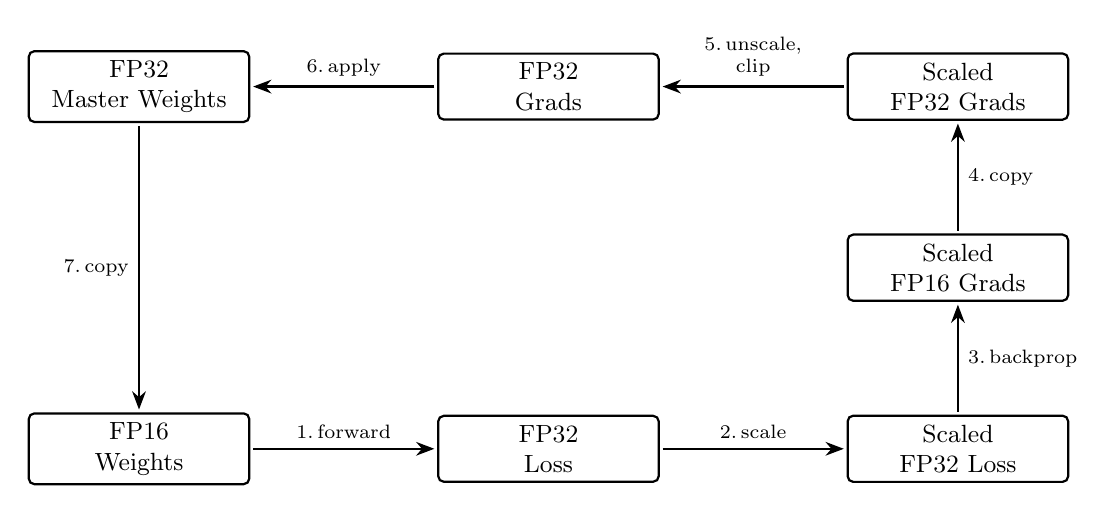
\begin{tikzpicture}[font=\footnotesize]
    % grid: columns x = 0, 5.2, 10.4;  rows y = 0, 2.3, 4.6
    \node[fsdpbox, minimum width=28mm] (master) at (0,    4.6) {FP32 \\ Master Weights};
    \node[fsdpbox, minimum width=28mm] (fp32g)  at (5.2,  4.6) {FP32 \\ Grads};
    \node[fsdpbox, minimum width=28mm] (sfp32g) at (10.4, 4.6) {Scaled \\ FP32 Grads};
    \node[fsdpbox, minimum width=28mm] (sfp16g) at (10.4, 2.3) {Scaled \\ FP16 Grads};
    \node[fsdpbox, minimum width=28mm] (sloss)  at (10.4, 0)   {Scaled \\ FP32 Loss};
    \node[fsdpbox, minimum width=28mm] (loss)   at (5.2,  0)   {FP32 \\ Loss};
    \node[fsdpbox, minimum width=28mm] (fp16w)  at (0,    0)   {FP16 \\ Weights};

    \draw[flow] (master) -- node[left, font=\scriptsize]{7.\,copy} (fp16w);
    \draw[flow] (fp16w)  -- node[above, font=\scriptsize]{1.\,forward} (loss);
    \draw[flow] (loss)   -- node[above, font=\scriptsize]{2.\,scale} (sloss);
    \draw[flow] (sloss)  -- node[right, font=\scriptsize]{3.\,backprop} (sfp16g);
    \draw[flow] (sfp16g) -- node[right, font=\scriptsize]{4.\,copy} (sfp32g);
    \draw[flow] (sfp32g) -- node[above, font=\scriptsize, align=center]{5.\,unscale,\\clip} (fp32g);
    \draw[flow] (fp32g)  -- node[above, font=\scriptsize]{6.\,apply} (master);
\end{tikzpicture}
\caption{The mixed-precision training cycle. \textsc{FP32} master state is the invariant; everything else is transient.}
\label{fig:mixed-precision}
\end{figure}

\subsection{Memory accounting}

Let $P$ denote the parameter count. Memory consumption splits into two qualitatively different pieces.

\begin{definition}[Static memory]
The memory occupied by the weights and by the persistent optimiser state. In the mixed-precision regime with Adam/AdamW, per parameter we require:
\begin{itemize}[leftmargin=2em, itemsep=0em]
    \item \textsc{FP32} master weights: $4$\,bytes;
    \item First and second Adam moments (both \textsc{FP32}): $4 + 4 = 8$\,bytes;
    \item \textsc{FP16} working copy of weights: $2$\,bytes;
    \item \textsc{FP16} gradients: $2$\,bytes.
\end{itemize}
This sums to $16$ bytes per parameter.
\end{definition}

\begin{definition}[Dynamic memory]
The memory occupied by \emph{activations}, whose magnitude depends on batch size, sequence length, and architectural details. It is retained across the forward pass so as to be consumed by the backward pass.
\end{definition}

\begin{example}[Llama 70B]
For $P = 7 \times 10^{10}$, static memory alone demands approximately
\[
    16 \cdot P = 16 \cdot 7 \times 10^{10} \text{ bytes} = 1.12 \text{ TB}.
\]
In particular, the optimiser state alone requires $8P \approx 560$\,GB---many times the capacity of any single GPU. \qed
\end{example}

The conclusion is unavoidable: above a certain scale, replication ceases to be an option. We must shard.

% ============================================================
\section{The Parallelism Landscape}
% ============================================================

Before examining \FSDP{} in detail, it is instructive to situate it within the broader taxonomy of parallelism strategies, each with characteristic trade-offs.

\subsection{Pipeline parallelism and the bubble}

In \emph{pipeline parallelism}, the model is partitioned along its depth: GPU~0 holds the first few layers, GPU~1 the next, and so on. A batch traverses the chain sequentially in the forward pass and in reverse during backpropagation.

\begin{figure}[ht]
\centering
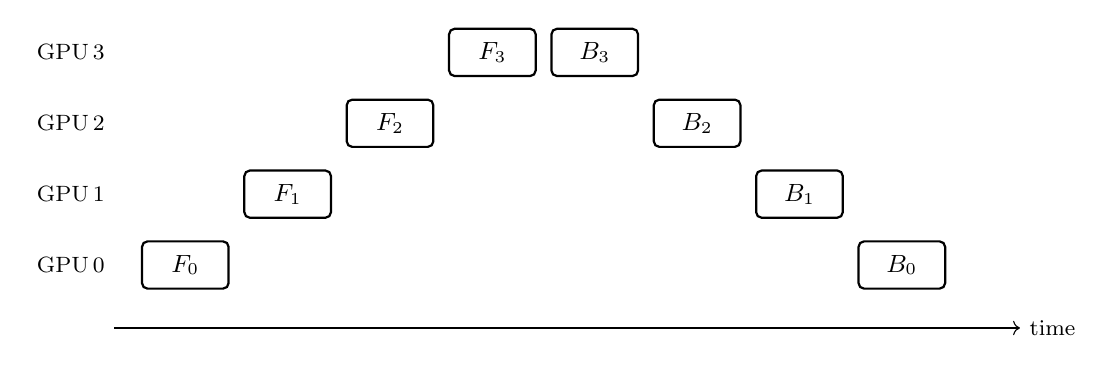
\begin{tikzpicture}[font=\footnotesize]
    % time axis, below all the rows
    \draw[->] (-0.3,-0.8) -- (11.2,-0.8) node[right] {time};

    \foreach \g in {0,1,2,3}
        \node[left] at (-0.3, \g*0.9) {GPU\,\g};

    % forward staircase
    \foreach \g/\x in {0/0.6, 1/1.9, 2/3.2, 3/4.5}
        \node[compbox, minimum width=11mm, minimum height=6mm]
            at (\x, \g*0.9) {$F_\g$};
    % backward staircase (reversed)
    \foreach \g/\x in {3/5.8, 2/7.1, 1/8.4, 0/9.7}
        \node[bwdbox, minimum width=11mm, minimum height=6mm]
            at (\x, \g*0.9) {$B_\g$};
\end{tikzpicture}
\caption{Pipeline parallelism across four devices. The diagonal staircase exposes the \emph{pipeline bubble}: while a late-stage GPU is still performing the first forward pass, earlier-stage GPUs sit idle.}
\label{fig:pipeline-bubble}
\end{figure}

The staircase pattern reveals the pathology: when GPU~3 is still computing $F_3$, GPU~0 has long finished $F_0$ and waits. This idle region---the \emph{pipeline bubble}---represents lost throughput.

\begin{remark}[Micro-batching]
The classical remedy is to split the global batch into several \emph{micro-batches} that march through the pipeline in overlapping fashion, shrinking the bubble without fully eliminating it. More recent \emph{zero-bubble} schedules, such as the \texttt{DualPipe} method developed by the DeepSeek team, further reorder forward and backward passes to eliminate idle time almost entirely---at the cost of considerable bookkeeping in the training code.
\end{remark}

\subsection{Tensor parallelism}

\emph{Tensor parallelism} partitions not the model's depth but its \emph{width}: every GPU holds a shard of every layer, and the matrix multiplications of each layer are carried out cooperatively. For the MLP block $Y = \mathrm{GeLU}(XA)\,B$ with $A = [A_1, A_2]$ and $B = [B_1; B_2]$ (split column-wise and row-wise respectively), each GPU computes a partial product and the results are summed. An analogous split applies to the attention block along the head dimension.

\begin{warning}
Unlike data or pipeline parallelism, the communication of tensor parallelism sits squarely on the critical path: the partial sums must be combined before the next layer can begin. The resulting latency cannot be hidden behind computation, which imposes a hard scaling ceiling---tensor parallelism rarely scales efficiently beyond a single node.
\end{warning}

\subsection{Distributed data parallelism (DDP)}

\DDP{} takes the opposite view. Every GPU stores a complete replica of the model and processes a disjoint shard of the data. During the forward pass the InfiniBand fabric is idle; only at the backward pass is communication required, and even there the synchronisation---an \AllReduce{} of gradients---can be overlapped with the computation of earlier-layer gradients.

The simplicity of \DDP{} is its strength. Its weakness is the memory footprint: every GPU carries the full 16$P$ bytes of static state, which is precisely what breaks at scale.

% ============================================================
\section{Fully Sharded Data Parallelism}
% ============================================================


\FSDP{} resolves the memory crisis of \DDP{} without surrendering its elegance. The central idea is a crisp one:

\begin{keyidea}
Partition the model's parameters, gradients, and optimiser states uniformly across the $N$ available GPUs. When a layer's full parameters are required for computation, gather them on the fly from across the cluster; the moment the computation finishes, discard the gathered copies and retain only the local shard.
\end{keyidea}

A useful mental picture---due to the lecturer---is that of a train laying its own track. Regardless of direction, we pick up the rails behind us and lay them in front just in time, so that only a short length of track ever exists at once.

\subsection{\texttt{FlatParameter} and the two states}

The atomic unit of \FSDP{} is the \texttt{FlatParameter}---a single one-dimensional buffer that concatenates the parameters of a designated \emph{\FSDP{} unit}. A \texttt{FlatParameter} exists in one of two states.

\begin{definition}[Sharded state]
The parameters are partitioned across the devices of a \emph{sharding group}, with each rank holding only a \emph{local shard}, possibly with trailing \emph{padding} to make sizes divisible by the group size. If one prints the weight of an \FSDP{} unit in the sharded state, one sees an empty tensor: from the unit's perspective, the size is effectively zero.
\end{definition}

\begin{definition}[Unsharded state]
The full parameters have been assembled on every device of the sharding group via an \AllGather{}, yielding the conventional dense tensor used for computation.
\end{definition}

\begin{figure}[ht]
\centering
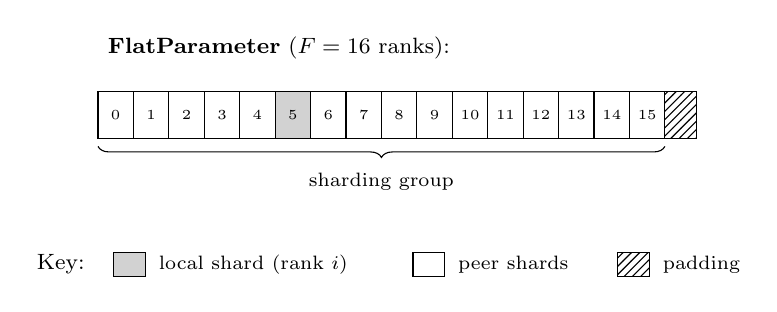
\begin{tikzpicture}[font=\footnotesize]
    % title
    \node[anchor=west] at (0, 1.15) {\textbf{FlatParameter} ($F=16$ ranks):};

    % highlight of the local shard (drawn first, under the outlines)
    \fill[gray!35] (5*0.45, 0) rectangle (6*0.45, 0.6);

    % the 16 shards
    \foreach \i in {0,...,15} {
        \draw (\i*0.45, 0) rectangle (\i*0.45+0.45, 0.6);
        \node[font=\tiny] at (\i*0.45+0.225, 0.3) {\i};
    }

    % trailing padding
    \draw[pattern=north east lines] (16*0.45, 0) rectangle (16*0.45+0.4, 0.6);

    % brace under the 16 shards
    \draw[decorate, decoration={brace, amplitude=4pt, mirror}]
        (0, -0.1) -- (16*0.45, -0.1)
        node[midway, below=6pt, font=\scriptsize] {sharding group};

    % legend
    \node[anchor=west] at (-0.9, -1.6) {Key:};
    \draw[fill=gray!35] (0.2, -1.75) rectangle (0.6, -1.45);
    \node[right, font=\scriptsize] at (0.65, -1.6) {local shard (rank $i$)};
    \draw (4.0, -1.75) rectangle (4.4, -1.45);
    \node[right, font=\scriptsize] at (4.45, -1.6) {peer shards};
    \draw[pattern=north east lines] (6.6, -1.75) rectangle (7.0, -1.45);
    \node[right, font=\scriptsize] at (7.05, -1.6) {padding};
\end{tikzpicture}
\caption{Full sharding across 16 GPUs. The \texttt{FlatParameter} is a concatenation of every parameter in the unit, split uniformly---with padding where necessary---into sixteen local shards.}
\label{fig:flatparam}
\end{figure}

\begin{remark}
A consequence of this flattening is that a \texttt{FlatParameter} in its sharded state is effectively just a vector of numbers, stripped of the tensor shapes that describe the underlying weight matrices. Those shapes are stored as metadata and reapplied at the moment of unsharding.
\end{remark}

\subsection{Units and the execution cycle}

The model is decomposed into a hierarchy of \emph{\FSDP{} units}. The outermost unit typically wraps the embedding and language-model head; inner units group the transformer blocks. Only registered units are sharded as a whole; the framework chooses when to gather based on module boundaries, not on individual operations.

The forward pass through one unit proceeds as:

\begin{center}
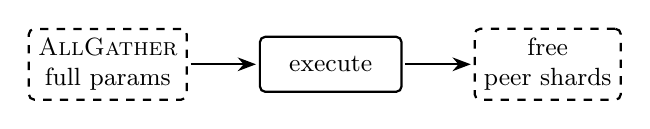
\begin{tikzpicture}[font=\footnotesize, node distance=9mm]
    \node[commbox] (ag) {\AllGather{} \\ full params};
    \node[compbox, right=of ag] (exec) {execute};
    \node[commbox, right=of exec] (fr) {free \\ peer shards};
    \draw[flow] (ag) -- (exec);
    \draw[flow] (exec) -- (fr);
\end{tikzpicture}
\end{center}

The backward pass augments this with gradient synchronisation:

\begin{center}
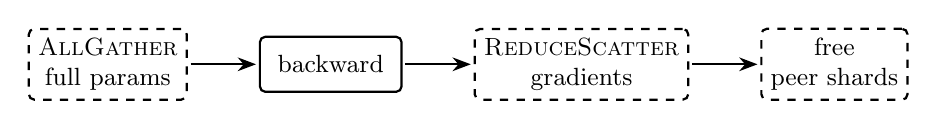
\begin{tikzpicture}[font=\footnotesize, node distance=9mm]
    \node[commbox] (ag) {\AllGather{} \\ full params};
    \node[bwdbox, right=of ag] (exec) {backward};
    \node[commbox, right=of exec] (rs) {\ReduceScatter{} \\ gradients};
    \node[commbox, right=of rs] (fr) {free \\ peer shards};
    \draw[flow] (ag) -- (exec);
    \draw[flow] (exec) -- (rs);
    \draw[flow] (rs) -- (fr);
\end{tikzpicture}
\end{center}

(Dashed boxes denote communication, solid boxes computation.) The crucial step is the \ReduceScatter{} at the end of the backward pass: it simultaneously averages gradients across the sharding group and redistributes them so that each rank ends up with only the gradients for the parameters it owns. The rank then performs an independent optimiser step on its own shard. No further communication is required for the update.

\subsection{Comparison with DDP}

\begin{figure}[H]
\centering
\resizebox{\textwidth}{!}{%
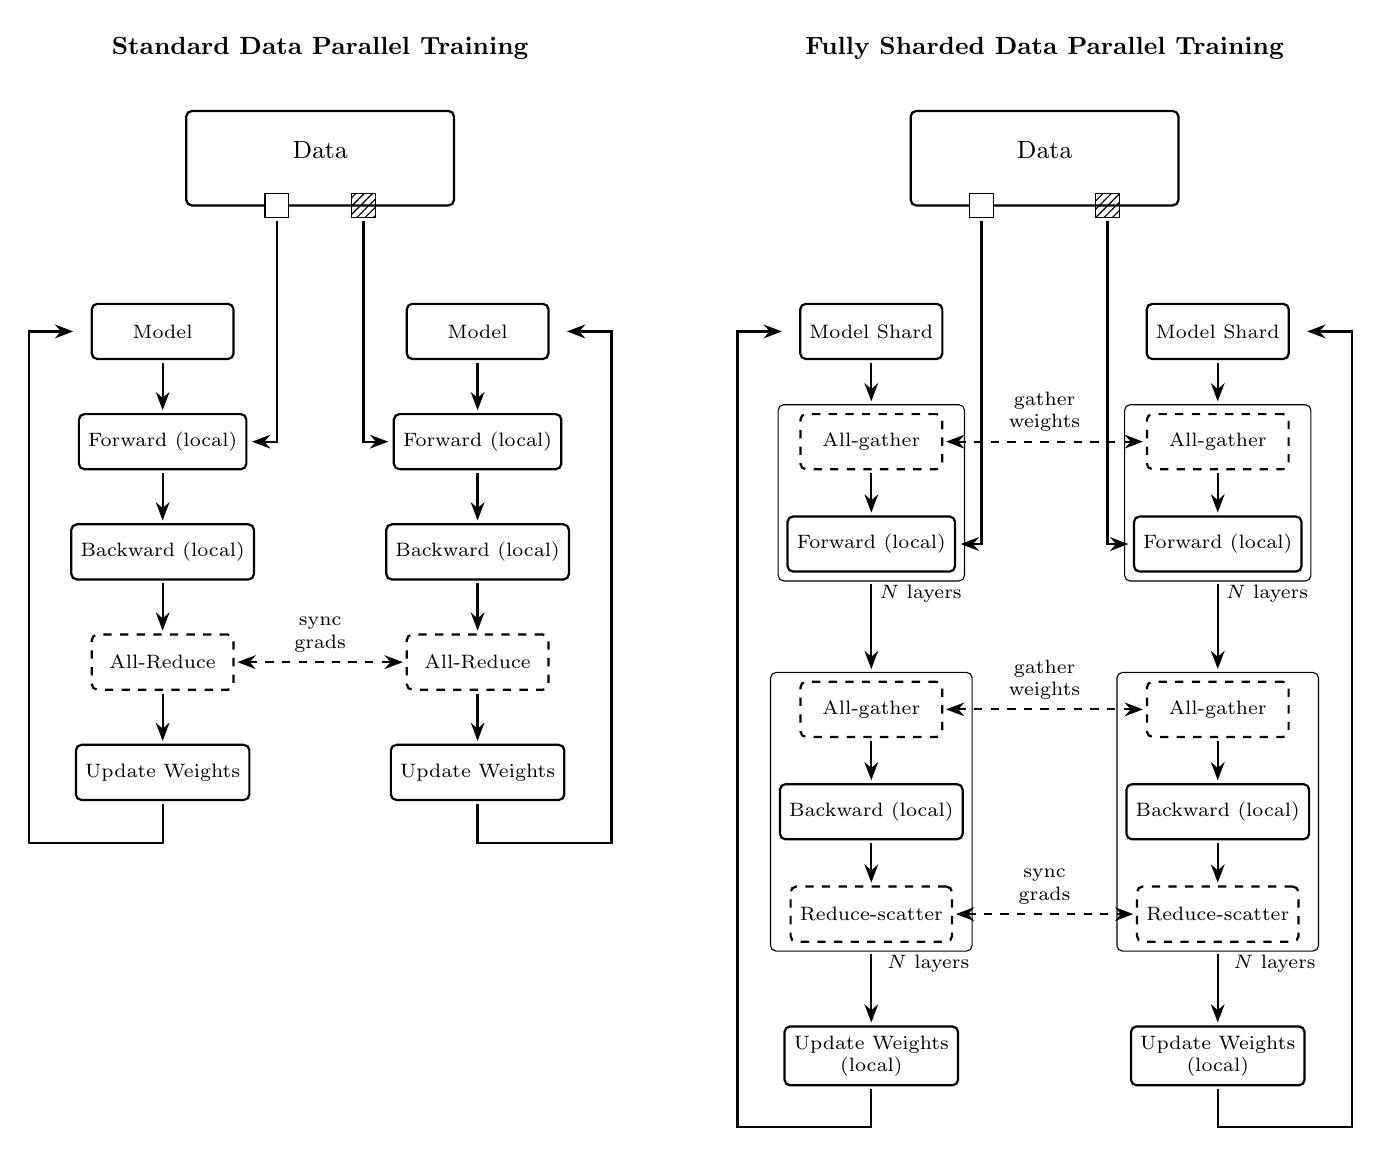
\begin{tikzpicture}[font=\scriptsize,
    bx/.style={fsdpbox, font=\scriptsize},
    bxc/.style={commbox, font=\scriptsize},
    frame/.style={draw, thin, rounded corners=2pt, inner sep=3pt},
    sync/.style={Stealth-Stealth, thick, dashed, shorten >=1pt, shorten <=1pt}]

    % ============ titles ============
    \node[font=\small\bfseries] at (2.0, 2.0)  {Standard Data Parallel Training};
    \node[font=\small\bfseries] at (11.2, 2.0) {Fully Sharded Data Parallel Training};

    % ============ DDP (two ranks, x = 0 and 4) ============
    \draw[rounded corners=2pt, thick] (0.3, 0) rectangle (3.7, 1.2);
    \node[font=\small] at (2.0, 0.7) {Data};
    \node[draw, minimum size=3mm, inner sep=0pt, fill=white] (dA) at (1.45, 0) {};
    \node[draw, minimum size=3mm, inner sep=0pt, pattern=north east lines] (dB) at (2.55, 0) {};

    \foreach \q/\x/\sg in {A/0/1, B/4/-1} {
        \pgfmathsetmacro{\xi}{\x+\sg*1.45}   % data line, inner side
        \pgfmathsetmacro{\xe}{\x+\sg*1.1}    % inner edge of Forward
        \pgfmathsetmacro{\xo}{\x-\sg*1.7}    % loop-back line, outer side
        \pgfmathsetmacro{\xm}{\x-\sg*1.1}    % outer edge of Model

        \node[bx]  (mo\q) at (\x, -1.6) {Model};
        \node[bx]  (fw\q) at (\x, -3.0) {Forward (local)};
        \node[bx]  (bw\q) at (\x, -4.4) {Backward (local)};
        \node[bxc] (ar\q) at (\x, -5.8) {All-Reduce};
        \node[bx]  (up\q) at (\x, -7.2) {Update Weights};

        \draw[flow] (mo\q) -- (fw\q);
        \draw[flow] (fw\q) -- (bw\q);
        \draw[flow] (bw\q) -- (ar\q);
        \draw[flow] (ar\q) -- (up\q);

        \draw[flow] (d\q.south) -- (\xi, -3.0) -- (\xe, -3.0);
        \draw[flow] (up\q.south) -- (\x, -8.1) -- (\xo, -8.1) -- (\xo, -1.6) -- (\xm, -1.6);
    }
    \draw[sync] (arA.east) -- node[above, align=center] {sync\\grads} (arB.west);

    % ============ FSDP (two ranks, x = 9 and 13.4) ============
    \draw[rounded corners=2pt, thick] (9.5, 0) rectangle (12.9, 1.2);
    \node[font=\small] at (11.2, 0.7) {Data};
    \node[draw, minimum size=3mm, inner sep=0pt, fill=white] (sA) at (10.4, 0) {};
    \node[draw, minimum size=3mm, inner sep=0pt, pattern=north east lines] (sB) at (12.0, 0) {};

    \foreach \q/\x/\sg in {A/9/1, B/13.4/-1} {
        \pgfmathsetmacro{\xi}{\x+\sg*1.4}
        \pgfmathsetmacro{\xe}{\x+\sg*1.1}
        \pgfmathsetmacro{\xo}{\x-\sg*1.7}
        \pgfmathsetmacro{\xm}{\x-\sg*1.1}

        \node[bx]  (smo\q) at (\x, -1.6) {Model Shard};

        % forward block, repeated for N layers
        \node[bxc] (sag1\q) at (\x, -3.0) {All-gather};
        \node[bx]  (sfw\q)  at (\x, -4.3) {Forward (local)};
        \node[frame, fit=(sag1\q)(sfw\q)] (fr1\q) {};
        \node[anchor=north east, inner sep=1pt] at (fr1\q.south east) {$N$ layers};

        % backward block, repeated for N layers
        \node[bxc] (sag2\q) at (\x, -6.4) {All-gather};
        \node[bx]  (sbw\q)  at (\x, -7.7) {Backward (local)};
        \node[bxc] (srs\q)  at (\x, -9.0) {Reduce-scatter};
        \node[frame, fit=(sag2\q)(sbw\q)(srs\q)] (fr2\q) {};
        \node[anchor=north east, inner sep=1pt] at (fr2\q.south east) {$N$ layers};

        \node[bx]  (sup\q) at (\x, -10.8) {Update Weights \\ (local)};

        \draw[flow] (smo\q.south) -- (fr1\q.north);
        \draw[flow] (sag1\q) -- (sfw\q);
        \draw[flow] (fr1\q.south) -- (fr2\q.north);
        \draw[flow] (sag2\q) -- (sbw\q);
        \draw[flow] (sbw\q) -- (srs\q);
        \draw[flow] (fr2\q.south) -- (sup\q.north);

        \draw[flow] (s\q.south) -- (\xi, -4.3) -- (\xe, -4.3);
        \draw[flow] (sup\q.south) -- (\x, -11.7) -- (\xo, -11.7) -- (\xo, -1.6) -- (\xm, -1.6);
    }
    \draw[sync] (sag1A.east) -- node[above, align=center] {gather\\weights} (sag1B.west);
    \draw[sync] (sag2A.east) -- node[above, align=center] {gather\\weights} (sag2B.west);
    \draw[sync] (srsA.east)  -- node[above, align=center] {sync\\grads}     (srsB.west);
\end{tikzpicture}}
\caption{The two paradigms contrasted, each shown on two GPUs; the hatched and plain squares are the two data shards. Dashed boxes and dashed arrows denote communication. \DDP{} performs a single \AllReduce{} per step; \FSDP{} replaces it with an \AllGather{} (forward), an \AllGather{} (backward), and a \ReduceScatter{}, repeated for each of the $N$ layers (units).}
\label{fig:ddp-vs-fsdp}
\end{figure}

% ============================================================
\section{Crash Course in NCCL}
% ============================================================


\FSDP{} rests on a small library of collective communication primitives, implemented by NVIDIA's \NCCL{} (pronounced \textit{``nickel''}) and exposed in PyTorch through \code{torch.distributed}. We review those we shall need.


A PyTorch distributed program begins with
\begin{center}
\code{torch.distributed.init\_process\_group(backend, init\_method, world\_size, rank, \dots)}
\end{center}
which admits several backends (Gloo, MPI, \NCCL{}); on GPU clusters, \NCCL{} is overwhelmingly the choice, exploiting \textsc{NVLink} for intra-node traffic and \textsc{InfiniBand} or \textsc{RoCE} for inter-node traffic. \NCCL{} abstracts the interconnect: the user writes collectives, and the library chooses an efficient realisation for the underlying topology.

\subsection{The primitives}

\begin{definition}[\AllReduce{}]
Given input tensors $\bm{x}_0, \bm{x}_1, \dots, \bm{x}_{K-1}$ on $K$ ranks, \AllReduce{} computes a reduction (typically sum) and broadcasts the result to every rank:
\[
    \text{out}_i \;=\; \bm{x}_0 \oplus \bm{x}_1 \oplus \cdots \oplus \bm{x}_{K-1}, \qquad i = 0, \dots, K-1.
\]
This is the workhorse of \DDP{} gradient synchronisation.
\end{definition}

\begin{definition}[\AllGather{}]
Each rank contributes a tensor $\bm{x}_i$ of size $N$; on return, every rank holds the concatenation
\[
    \text{out}_i \;=\; [\bm{x}_0, \bm{x}_1, \dots, \bm{x}_{K-1}], \qquad i = 0, \dots, K-1,
\]
of total size $KN$, ordered by rank index.
\end{definition}

\begin{definition}[\ReduceScatter{}]
The formal dual of \AllGather{}. Each rank contributes a tensor of size $KN$; the operation computes the rank-wise reduction and then scatters the result so that rank~$i$ retains only its $i$-th chunk of size $N$. Equivalently, \AllReduce{} $=$ \ReduceScatter{} followed by \AllGather{}.
\end{definition}

\begin{observation}
It is no accident that \FSDP{}'s two communication steps---\AllGather{} in the forward pass and \ReduceScatter{} at the end of the backward pass---compose, in aggregate, to the \AllReduce{} performed by \DDP{}. \FSDP{} does not avoid the communication; it spreads it out and, in doing so, buys itself the ability to discard full-size parameters between layers.
\end{observation}

% ============================================================
\section{Memory Accounting and the ``Almost Free'' Claim}
% ============================================================

\subsection{Bytes on the wire}

How much more does \FSDP{} communicate than \DDP{}? Consider a model of parameter count $P$ distributed over $N$ ranks.

\begin{itemize}[leftmargin=2em]
    \item \DDP{}: one \AllReduce{} of $P$ gradients per step.
    \item \FSDP{}: one \AllGather{} of $P$ parameters in the forward pass, a second \AllGather{} of $P$ parameters in the backward pass, and one \ReduceScatter{} of $P$ gradients.
\end{itemize}

To a first approximation (and modulo the fact that \AllReduce{} already decomposes into a reduce-scatter and an all-gather internally), \FSDP{} transmits roughly \emph{one and a half times} as many bytes as \DDP{}. The overhead is real but modest.

\subsection{Static footprint: Llama 70B on 128 GPUs}

Set $P = 70 \times 10^9$, $N = 128$, and suppose weights and gradients in \textsc{BF16} (2 bytes), Adam moments in \textsc{FP32} (8 bytes total per parameter). The per-GPU static footprint is
\begin{align}
    \text{weights}    &\;\approx\; \frac{70 \times 10^9 \cdot 2}{128} \;\approx\; 1.1 \text{ GB}, \\
    \text{gradients}  &\;\approx\; \frac{70 \times 10^9 \cdot 2}{128} \;\approx\; 1.1 \text{ GB}, \\
    \text{optimiser}  &\;\approx\; \frac{70 \times 10^9 \cdot 8}{128} \;\approx\; 4.4 \text{ GB}.
\end{align}
Dense replicas would have required $140 + 140 + 560 = 840$ GB per GPU---wholly impossible. \FSDP{} reduces this to under $7$ GB per GPU.

\subsection{Dynamic footprint: the gather buffers}

To the static shards we must add the transient \AllGather{} buffers that hold a unit's full parameters during computation. For Llama~70B with transformer-block units of roughly $0.9 \times 10^9$ parameters each, the buffers cost
\[
    \underbrace{0.9 \times 10^9 \cdot 2}_{\text{weight buffer}} \;+\; \underbrace{0.9 \times 10^9 \cdot 2}_{\text{gradient buffer}} \;=\; 3.6 \text{ GB per unit}.
\]
Once computation completes, both buffers are released back into the allocator.

\begin{remark}
At $N = 1280$ the static shards become essentially negligible, and the gather buffers dominate. It is natural to ask: \emph{why two buffers?} The answer lies in prefetching---we shall return to it in Section~\ref{sec:prefetch}.
\end{remark}

% ============================================================
\section{Profiling, Streams, and the Anatomy of Overlap}
% ============================================================


The ``almost free'' character of \FSDP{} is not automatic. It depends on the successful overlap of communication with computation---a phenomenon best understood, and best debugged, through the PyTorch profiler.

\subsection{The profiler}

Wrapping a forward pass in a context manager suffices to capture a complete trace:

\begin{center}
\begin{minipage}{0.88\textwidth}
\small
\begin{verbatim}
    device = 'cuda'
    activities = [ProfilerActivity.CPU, ProfilerActivity.CUDA]

    model  = models.resnet18().to(device)
    inputs = torch.randn(5, 3, 224, 224).to(device)

    with profile(activities=activities) as prof:
        model(inputs)

    prof.export_chrome_trace("trace.json")
\end{verbatim}
\end{minipage}
\end{center}

The resulting \texttt{trace.json} may be opened in \code{chrome://tracing}, revealing a Gantt-chart view of the execution: the CPU thread dispatches operators; the GPU streams execute kernels; and the gaps between them tell their own story.

\begin{figure}[ht]
\centering
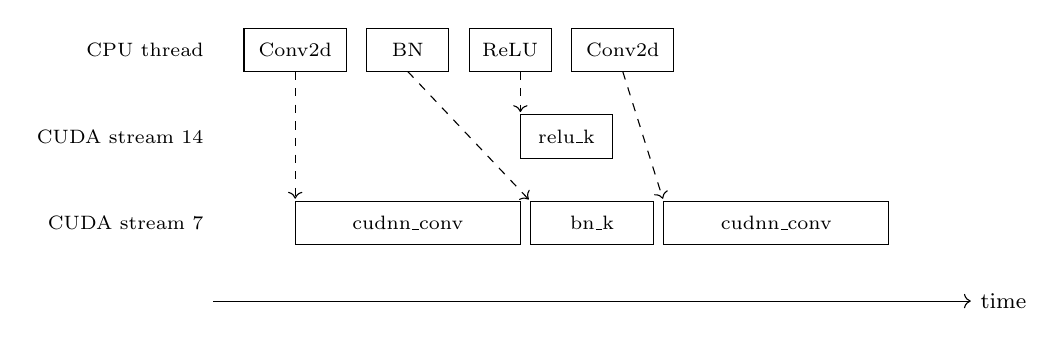
\begin{tikzpicture}[font=\footnotesize, x=1.3cm, y=1.1cm]
    % time axis, below all rows
    \draw[->] (0, 0.1) -- (7.4, 0.1) node[right] {time};

    \node[left, font=\scriptsize] at (0, 3) {CPU thread};
    \node[left, font=\scriptsize] at (0, 2) {CUDA stream 14};
    \node[left, font=\scriptsize] at (0, 1) {CUDA stream 7};

    % CPU operators (short: dispatch only)
    \foreach \a/\b/\l in {0.3/1.3/Conv2d, 1.5/2.3/BN, 2.5/3.3/ReLU, 3.5/4.5/Conv2d}
        \draw (\a, 2.75) rectangle (\b, 3.25) node[midway, font=\scriptsize] {\l};

    % GPU kernels, stream 14
    \draw (3.0, 1.75) rectangle (3.9, 2.25) node[midway, font=\scriptsize] {relu\_k};

    % GPU kernels, stream 7 (FIFO queue)
    \foreach \a/\b/\l in {0.8/3.0/cudnn\_conv, 3.1/4.3/bn\_k, 4.4/6.6/cudnn\_conv}
        \draw (\a, 0.75) rectangle (\b, 1.25) node[midway, font=\scriptsize] {\l};

    % dispatch arrows (CPU op -> kernel start): none crosses a box
    \draw[->, dashed, shorten >=1pt] (0.8, 2.75) -- (0.8, 1.25);
    \draw[->, dashed, shorten >=1pt] (1.9, 2.75) -- (3.1, 1.25);
    \draw[->, dashed, shorten >=1pt] (3.0, 2.75) -- (3.0, 2.25);
    \draw[->, dashed, shorten >=1pt] (4.0, 2.75) -- (4.4, 1.25);
\end{tikzpicture}
\caption{A schematic profiler trace: CPU operators are dispatched asynchronously onto CUDA streams, which execute in parallel. Dashed arrows denote dispatch; the horizontal axis is wall time. Note that the CPU is already finished dispatching while the GPU is still working through the queue of stream~7.}
\label{fig:profiler}
\end{figure}

\subsection{Streams, queues, and implicit asynchrony}

A CUDA \emph{stream} is a FIFO queue of kernels. Submitting a kernel to a stream is a near-instantaneous operation---the kernel is \emph{enqueued}, not executed. It runs only when its stream's previous kernels have completed and the GPU has spare streaming multiprocessors (SMs) to service it.

This explains a common source of surprise. If a Python thread launches ten thousand heavy matrix multiplies, the Python call returns almost immediately---the CPU has merely dispatched ten thousand entries onto a stream. The GPU will grind through them in due course; the CPU is free to continue submitting more work.

Two practical consequences follow.

\begin{enumerate}[leftmargin=2em, itemsep=0.15em]
    \item \emph{The CPU must stay ahead of the GPU} to keep streams saturated---if the CPU blocks, the GPU will eventually run out of queued work and stall.
    \item \emph{Multiple streams can execute concurrently}, provided they are independent. Two kernels that each use only $50\%$ of the SMs can, in principle, run in parallel if scheduled on separate streams. This is the mechanism by which \NCCL{} collectives are made to overlap with computation.
\end{enumerate}


When two streams have a data dependency, explicit synchronisation is required. If stream~7 contains a convolution that consumes the output of a kernel on stream~32, the profiler will show stream~7 waiting at the dependency point until stream~32 drains. Misplaced synchronisations are a classic cause of idle GPU time.

\subsection{Where \NCCL{} steals SMs}

\NCCL{} collectives are themselves CUDA kernels, and they consume SMs. Happily, they usually consume very few: an \AllGather{} may occupy a single-digit percentage of the chip, leaving the rest available for matrix multiplies. This is why overlap is possible at all. Not every implementation is equally parsimonious, however---low-quality collective implementations sometimes require copying small fragments of data (kilobytes, or even hundreds of bytes) through a fixed memory address, demanding an immediate follow-up copy to free the address for the next fragment. Technologies like \textsc{SHARP} (Scalable Hierarchical Aggregation and Reduction Protocol) alleviate this by performing the reduction within the network fabric itself, removing the need for GPU cores to participate in arithmetic at all.

% ============================================================
\section{Prefetching: Hiding the Gather}
\label{sec:prefetch}
% ============================================================


Even with stream-level concurrency, na\"ive scheduling of \FSDP{} leaves the GPU idle. The forward pass of unit $i$ cannot begin until its \AllGather{} completes; if the \AllGather{} is only enqueued when the preceding computation finishes, the chip sits waiting.

\subsection{Implicit forward prefetching}

Because the CPU thread runs \emph{ahead} of the GPU---submitting kernels many microseconds in advance of their execution---the \AllGather{} of unit $i+1$ can be enqueued on the communication stream \emph{while} the computation stream is still processing unit~$i$. The two streams proceed in parallel: communication hides behind computation. This is \emph{implicit forward prefetching}, and it is essentially free---a consequence of asynchronous dispatch.

\subsection{Explicit forward prefetching}

For models with irregular or dynamic control flow---Mixture-of-Experts architectures being the paradigmatic case---implicit prefetching is insufficient: the scheduler cannot know in advance which unit will be visited next. PyTorch exposes an explicit option:
\begin{center}
\code{model = FSDP(model, auto\_wrap\_policy=..., forward\_prefetch=True)}
\end{center}
The mechanism operates in two phases.
\begin{enumerate}[leftmargin=2em, itemsep=0.15em]
    \item \emph{Recording.} During the first forward pass, \FSDP{} records the order in which \AllGather{}s were issued.
    \item \emph{Proactive submission.} In all subsequent iterations, when unit $i$ begins its \AllGather{}, the pre-forward hook of unit $i+1$ simultaneously submits \emph{its} \AllGather{} to the communication stream.
\end{enumerate}
Naturally, this works only if the execution order is \emph{static}---the same units invoked in the same order every step. For genuinely dynamic models, more sophisticated dynamic-assembly strategies are required.

\subsection{Explicit backward prefetching}

In the backward pass the situation is more subtle, and here explicit prefetching is \emph{essential}---without it, overlap drops to zero. The reason is a subtle ordering issue on a single communication queue.

Suppose we are at layer $i$ of the backward pass. Two communications are pending: the \ReduceScatter{} of gradients for layer $i$ (just computed), and the \AllGather{} of parameters for layer $i-1$ (about to be needed). If we na\"ively enqueue the \ReduceScatter{} first, the \AllGather{} must wait behind it---and the backward computation of layer $i-1$ cannot even begin.

The correct order is the opposite: \emph{issue the \AllGather{} for $i-1$ first, then the \ReduceScatter{} for $i$}. The \AllGather{} races ahead on the communication stream; the \ReduceScatter{} can complete at its leisure while the compute stream works on layer $i-1$.

\begin{center}
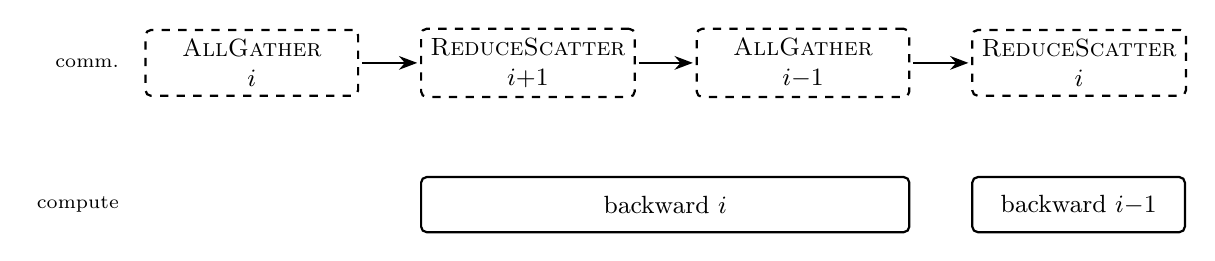
\begin{tikzpicture}[font=\scriptsize]
    % communication queue (top row): 4 boxes of width 27mm, pitch 35mm
    \node[left] at (-0.2, 0) {comm.};
    \node[commbox, minimum width=27mm, anchor=west] (ag1) at (0,    0) {\AllGather{} \\ $i$};
    \node[commbox, minimum width=27mm, anchor=west] (rsp) at (3.5,  0) {\ReduceScatter{} \\ $i{+}1$};
    \node[commbox, minimum width=27mm, anchor=west] (ag2) at (7.0,  0) {\AllGather{} \\ $i{-}1$};
    \node[commbox, minimum width=27mm, anchor=west] (rs)  at (10.5, 0) {\ReduceScatter{} \\ $i$};
    \draw[flow] (ag1) -- (rsp);
    \draw[flow] (rsp) -- (ag2);
    \draw[flow] (ag2) -- (rs);

    % compute row (bottom): backward i overlaps RS(i+1) and AG(i-1)
    \node[left] at (-0.2, -1.8) {compute};
    \node[bwdbox, minimum width=62mm, anchor=west] (bi1) at (3.5,  -1.8) {backward $i$};
    \node[bwdbox, minimum width=27mm, anchor=west] (bi2) at (10.5, -1.8) {backward $i{-}1$};
\end{tikzpicture}
\end{center}

The two-buffer requirement we noted earlier is now explained: the system must hold parameters for the currently executing layer \emph{and} parameters being prefetched for the next, simultaneously.

\begin{warning}
A CPU running too far ahead of the GPU can overshoot: queues may fill, allocations cascade, and synchronisation can fail subtly. Prefetching is a matter of balance, not maximal aggression.
\end{warning}

% ============================================================
\section{Overlap: The Complete Picture}
% ============================================================

We may now assemble the full overlap diagram. On a single forward-backward step, three agents operate in concert: the CPU (orchestrating), the GPU compute stream (running kernels), and the GPU communication stream (moving parameters and gradients).

\begin{figure}[ht]
\centering
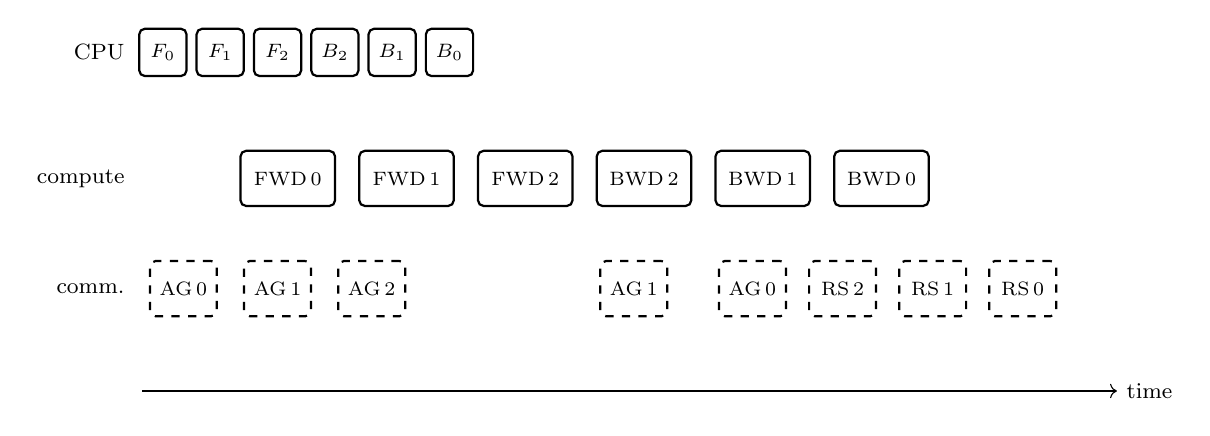
\begin{tikzpicture}[font=\scriptsize, x=1.04cm]
    % time axis
    \draw[->] (0, -0.7) -- (11.9, -0.7) node[right, font=\footnotesize] {time};

    % row labels
    \node[left, font=\footnotesize] at (-0.1, 3.6) {CPU};
    \node[left, font=\footnotesize] at (-0.1, 2.0) {compute};
    \node[left, font=\footnotesize] at (-0.1, 0.6) {comm.};

    % CPU row: all dispatches finish early (the CPU runs ahead)
    \foreach \x/\l in {0.25/F_0, 0.95/F_1, 1.65/F_2, 2.35/B_2, 3.05/B_1, 3.75/B_0}
        \node[fsdpbox, minimum width=6mm, minimum height=6mm, inner sep=1pt, font=\scriptsize]
            at (\x, 3.6) {$\l$};

    % compute stream
    \foreach \cx/\l in {1.775/FWD\,0, 3.225/FWD\,1, 4.675/FWD\,2}
        \node[compbox, minimum width=12mm, minimum height=7mm, font=\scriptsize]
            at (\cx, 2.0) {\l};
    \foreach \cx/\l in {6.125/BWD\,2, 7.575/BWD\,1, 9.025/BWD\,0}
        \node[bwdbox, minimum width=12mm, minimum height=7mm, font=\scriptsize]
            at (\cx, 2.0) {\l};

    % communication stream
    \foreach \cx/\l in {0.5/AG\,0, 1.65/AG\,1, 2.8/AG\,2,
                        6.0/AG\,1, 7.45/AG\,0,
                        8.55/RS\,2, 9.65/RS\,1, 10.75/RS\,0}
        \node[commbox, minimum width=8.5mm, minimum height=7mm, inner sep=2pt, font=\scriptsize]
            at (\cx, 0.6) {\l};
\end{tikzpicture}
\caption{The idealised \FSDP{} pipeline for three units. Communication operations (\AllGather{} and \ReduceScatter{}, dashed) on the communication stream overlap with matrix-multiply kernels on the compute stream. The CPU races ahead of both, having enqueued the whole step before the GPU is half-way through it. In the backward pass the \AllGather{} for the next layer is issued before the pending \ReduceScatter{}.}
\label{fig:overlap}
\end{figure}

When all three are in balance, the total wall-clock time satisfies
\[
    T_{\text{step}} \;\approx\; \max\bigl(T_{\text{compute}}, \; T_{\text{communication}}\bigr).
\]
In the compute-bound regime $T_{\text{communication}} \ll T_{\text{compute}}$, and \FSDP{} runs almost as fast as \DDP{}.

\subsection{What can go wrong}

The qualifier \emph{almost} earns its keep through a handful of failure modes.

\begin{itemize}[leftmargin=2em, itemsep=0.15em]
    \item \textbf{Non-uniform sharding.} If layers vary wildly in parameter count or in compute cost, some steps will be communication-bound and others compute-bound. The schedule cannot overlap both regimes simultaneously.
    \item \textbf{Slow interconnect.} The speed of \AllGather{} and \ReduceScatter{} is set by the network; on clusters with poor topology, communication cannot finish in time.
    \item \textbf{Small units.} If \FSDP{} units are too small, the per-unit overhead of launching an \AllGather{} dominates. The framework amortises best on units of a few hundred million parameters.
    \item \textbf{Stale \NCCL{} versions.} \NCCL{} receives substantive optimisations with each release. An old version can quietly cap performance.
\end{itemize}

% ============================================================
\section{Flavours of Sharding}
% ============================================================


\FSDP{} offers a family of sharding strategies, trading memory savings for communication bandwidth along a Pareto frontier.

\subsection{\texttt{NO\_SHARD}}

Equivalent to \DDP{}. Every rank holds the full model; gradients are synchronised by \AllReduce{}. No sharding of any kind. Useful as a baseline and as a degenerate case of the \FSDP{} wrapper, whose implementation is often more robust than the legacy \code{torch.nn.DataParallel}.

\subsection{\texttt{SHARD\_GRAD\_OP}}

Shards gradients and optimiser states but \emph{not} the \textsc{BF16} working copy of weights: once gathered for the forward pass, the weights are kept resident through the backward pass. The cost is an additional $2P$ bytes of memory per rank; the benefit is one fewer \AllGather{} per step---the forward-pass gather is reused---bringing the total data moved back in line with \DDP{}.

This strategy works well up to roughly $30$B parameters, beyond which the extra weight copy becomes itself the bottleneck.

\subsection{\texttt{FULL\_SHARD}}

The most aggressive strategy. Weights, gradients, and optimiser states are all sharded. Memory per rank is minimised; the full communication cost (two \AllGather{}s and one \ReduceScatter{}) is paid each step. This is the appropriate choice for very large models.

\subsection{\texttt{HYBRID\_SHARD}}

A compromise that exploits hierarchical cluster topology. The $N$ GPUs are divided into $G$ groups of size $N/G$ (typically $256$ or $512$). Within a group, \FSDP{} operates in \texttt{FULL\_SHARD} mode; across groups, the framework maintains replicas and synchronises them with \AllReduce{}.

\begin{figure}[ht]
\centering
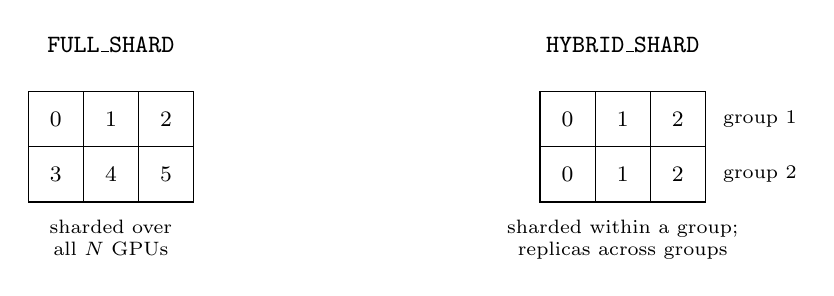
\begin{tikzpicture}[font=\footnotesize]
    % ---- FULL_SHARD: 6 GPUs, 6 different shards ----
    \begin{scope}
        \node[font=\small\bfseries] at (1.05, 2.0) {\texttt{FULL\_SHARD}};
        \foreach \x in {0,1,2} \foreach \y in {0,1} {
            \pgfmathtruncatemacro{\n}{\x + 3*(1-\y)}
            \draw (\x*0.7, \y*0.7) rectangle (\x*0.7+0.7, \y*0.7+0.7);
            \node at (\x*0.7+0.35, \y*0.7+0.35) {\n};
        }
        \node[below, font=\scriptsize, align=center] at (1.05, -0.1) {sharded over\\ all $N$ GPUs};
    \end{scope}
    % ---- HYBRID_SHARD: 2 groups of 3 GPUs, replicated ----
    \begin{scope}[xshift=6.5cm]
        \node[font=\small\bfseries] at (1.05, 2.0) {\texttt{HYBRID\_SHARD}};
        \foreach \x in {0,1,2} \foreach \y in {0,1} {
            \draw (\x*0.7, \y*0.7) rectangle (\x*0.7+0.7, \y*0.7+0.7);
            \node at (\x*0.7+0.35, \y*0.7+0.35) {\x};
        }
        \node[right, font=\scriptsize] at (2.2, 1.05) {group 1};
        \node[right, font=\scriptsize] at (2.2, 0.35) {group 2};
        \node[below, font=\scriptsize, align=center] at (1.05, -0.1) {sharded within a group;\\ replicas across groups};
    \end{scope}
\end{tikzpicture}
\caption{Each square is a GPU and its number is the index of the shard it holds. In \texttt{HYBRID\_SHARD} the rows are sharding groups: each row holds the full sharded model, and identical numbers mark replicas of the same shard. Only \AllReduce{} traffic crosses the slow inter-group link.}
\label{fig:hybrid}
\end{figure}

The motivation is topological. In a cluster of $20{,}480$ GPUs, a global \AllGather{} across all ranks crosses every switch in the fabric. By confining the sharding \AllGather{}s to local groups---each contained within a Slimmed Fat-Tree (SFT) subtree---only the cheaper inter-replica \AllReduce{} crosses the cluster-wide links. The arrangement maps neatly onto real interconnects.

\begin{warning}
\texttt{HYBRID\_SHARD} is a specialist's instrument. Its configuration is intricate and its advantages manifest only at extreme scale---typically above $2{,}000$ GPUs. For clusters below that threshold, standard \texttt{FULL\_SHARD} is both simpler and faster.
\end{warning}

% ============================================================
\section{DeepSpeed ZeRO: The Intellectual Ancestor}
% ============================================================

\FSDP{} did not arrive ex nihilo; it was preceded, and in many respects prefigured, by Microsoft's \textbf{DeepSpeed ZeRO} (Zero Redundancy Optimizer). ZeRO organises its own optimisations into stages of increasing aggressiveness, which correspond closely to the flavours above:

\begin{description}[leftmargin=2.2em, style=nextline]
    \item[ZeRO-0] No sharding; equivalent to \DDP{}.
    \item[ZeRO-1] Shard optimiser states only.
    \item[ZeRO-2] Shard optimiser states and gradients. Corresponds to \texttt{SHARD\_GRAD\_OP}.
    \item[ZeRO-3] Shard optimiser states, gradients, and parameters. Corresponds to \texttt{FULL\_SHARD}.
\end{description}

DeepSpeed additionally offers features not present in vanilla \FSDP{}---gradient compression, exotic offloading modes, and more---at the cost of a considerably more complex API. \FSDP{}, particularly in its \FSDP{}2 incarnation, has largely caught up while remaining closer in spirit to native PyTorch.

\begin{remark}[\FSDP{}2]
The second-generation implementation (\FSDP{}2) is architecturally distinct from the original: it shards parameters \emph{per-parameter} rather than by flattening them into a single \texttt{FlatParameter} per unit, and it interoperates cleanly with \code{torch.compile} and \texttt{DTensor}. Raw throughput is comparable to \FSDP{}1; the architectural gains are in composability and elegance. For new projects, \FSDP{}2 is the recommended starting point. See the RFC at \url{https://github.com/pytorch/pytorch/issues/114299}.
\end{remark}

% ============================================================
\section{Activation Checkpointing}
% ============================================================

Static sharding addresses weights, gradients, and optimiser states, but leaves untouched the dynamic footprint of \emph{activations}. For deep networks with long sequences, these can dwarf the static state. The remedy is \emph{activation checkpointing} (also called gradient checkpointing): during the forward pass, only a subset of activations is retained; the rest are recomputed on demand during the backward pass.

\begin{remark}
Activation checkpointing composes naturally with \FSDP{}, and the two together extend the trainable scale by an order of magnitude. The cost is an approximately $20\%$ computational overhead, corresponding to the recomputed forward passes on the critical path. The tradeoff is almost always worthwhile for memory-constrained training of very deep models.
\end{remark}

\end{document}